\documentclass{article}

\title{2.4 Sensitivity of Optimisation Algorithms to Initial Conditions}
\date{2020-03-23}


\usepackage{amsfonts}
\usepackage{amsmath}
\usepackage{amssymb}
\usepackage{graphicx}
\usepackage{subcaption}
\usepackage{listings}


\begin{document}

\maketitle

\section{Introduction}

In modern statistics and machine learning, it is common to derive estimators and make decisions by minimising some objective function $f$. Often this cannot be solved in closed form and so it is common place to use iterative optimisation algorithms to attempt to find approximate minimisers. This report aims to explore and further understand the sensitivity of our optimisation algorithm to their initialisation, in the case that multiple minima exist.

\newpage

\section{Gradient descent}

Throughout this project the optimisation algorithm of study will be the gradient descent algorithm defined as follows. Define a differentiable objective function $f : \textbf{D} \to \textbf{R} $ with domain $\textbf{D} \subseteq \textbf{R}^d$ , $d \geq 1$, an initial point $x_0 \in \textbf{D}$, and a step size $h > 0$. The iterates of the algorithm are then defined as 
\begin{equation}
x_t=x_{t-1}-h \nabla f(x_{t-1}), \indent  \text{for } t \in \{ 1,2,... \} .
\end{equation}
In what follows, we will focus our attention on minimisation of the ‘double-well’ toy function $f_\theta$, defined for $\theta \in (0, \pi)$ by
\begin{equation}
f_\theta : [-1,1] \to \textbf{R}, \indent x \mapsto (x^2 - 3/4)^2 - x \cos(\theta).
\end{equation}

\subsection{Question 1}

The stationary points of $f_\theta$ can be found by solving the following eqation set to zero.
\begin{equation}
f_\theta'(x) = 4x^3-3x- \cos(\theta)
\end{equation}
We can spot the first solution via use of the known triple angle formula, $\cos(3A)=4\cos^3(A)-3\cos(A)$, then using $x=\cos(A)=\cos(\theta / 3)$ gives the required result. Then using polynomial division and then the quadratic formula (and some simple trig identities) we arrive at the second and third solutions to the cubic. These solutions are displayed below. 
\begin{equation}
x_1 = cos(\theta/3)
\end{equation}
\begin{equation}
x_2 =(1/2)(-\cos(\theta/3)+ \sqrt{3}\sin(\theta/3))=-\sin \left( \frac{\pi}{6}-\frac{\theta}{3} \right)
\end{equation}
\begin{equation}
x_3 =(1/2)(-\cos(\theta/3)- \sqrt{3}\sin(\theta/3))=-\sin \left( \frac{\pi}{6}+\frac{\theta}{3} \right)
\end{equation}
We can then classify these stationary points by considering the sign of 
\begin{equation}
f_\theta ''(x_i)=12x_i^2-3. 
\end{equation}
First lets find the roots of this equation for $i=1$. Trivially we see $\theta = \pm \pi + 3n \pi $ with $n \in \mathbb{Z} $ is a complete set of roots to this equation. We can note that $f_\theta''$ is clearly continuous in $x$, $f_\theta''(x_1|_{\theta=0})=9$ (by direct calculation) and that by above the first root on the right of $\theta=0$ is $\theta=\pi$. Therefore, we can conlude by use of Intermediate Value Theorem (stated in appendicies on page~\pageref{IVT}) that $f_\theta''(x_1)>0,  \forall \theta \in (0,\pi)$, otherwise, we arise at a the conlustion a new root must exist outside of the set of solutions already found, a contradiction. As a result we can conclude $x_1$ is a local minimum of the function.\\
\\
We can similarly sove equation (7) for $i=2$ and $3$ to give complete solution sets of $\{0+3n\pi,\pi+3n\pi\}$ and $\{0+3n\pi,-\pi+3n\pi\}$ respectively, with $n \in \mathbb{Z} $. We can note by direct calculation the values $f_\theta''(x_2|_{\theta=\pi/2})=-3$ and $f_\theta''(x_3|_{\theta=\pi/2})=6$. Then using a similar arguement to the $i=1$ case we can conclude that $f_\theta''(x_2)<0$ and $f_\theta''(x_3)>0$ for $\theta \in (0,\pi)$. Thus, for the relevant values of $\theta$ we can conclude $x_2$ is a local maximum and $x_3$ is a local minimum. \\

\subsection{Question 2}
Taking $\theta=\frac{\pi}{6}$, $h=0.01$, and running the gradient descent algorithm described earlier (code found on page~\pageref{subsec:Program 1}) over $1000$ steps from initial points $x_0 \in \{\frac{k}{50}\}_{k=-50}^{50}$. Running '$>>>$grad$\_$descent' will give the following results.
\begin{center}
\begin{tabular}{ c c c } 
 k & Value of $x_{1000}$ & $|x_{1000}-x_{999}|$ \\
\hline 
 -50 & -0.642787610032 & $7.23132 \times 10^{-12}$\\ 
 -49 & -0.642787610040 & $7.07911 \times 10^{-12}$ \\
 \vdots & \vdots \\
-18 & -0.642787586093 & $4.71198 \times 10^{-10}$ \\
-17 & 0.984807753012 & $0.0$ \\
\vdots & \vdots \\
49 & 0.984807753012 & $0.0$ \\
50 & 0.984807753012 & $0.0$ \\ 
\end{tabular}
\end{center}
It is clear from the table then that the algorithm converges to two local minima at approximately $x=-0.643$ and $x=0.985$. These match agaist the analytic solutions that give for $\theta=\frac{\pi}{6}$, $x_1 = 0.984807753012$ and $x_3= -0.632787609687$ suggesting high accuracy of the algorithm. We can also note that the point at which the algorithm switches from finding $x_1$, to finding $x_3$, occurs between $x=-\frac{17}{50}=-0.34$ and $x=-\frac{18}{50}=-0.36$, and that $x_2=-0.342020143326$ which lies directly between the two steps. This suggests that the point at which the specific minimum found by the algorithm changes is related to its position relative to local maximums of the function. 

\section{The Monte Carlo Method}

Define the following quantities and random variables for some function $g$ and independent identically distributed random variables $X, \{X^i\}_{i=1}^N$.
\begin{equation}
\nu =\textbf{E} [g(X)]
\end{equation}
\begin{equation}
\hat{\nu}_N \triangleq \frac{1}{N} \sum_{i=1}^Ng(X^i).
\end{equation}

\subsection{Question 3}
\paragraph{Theorem}
$\hat{\nu}_N$ is unbiased for $\nu$.
\paragraph{Proof}
$\hat{\nu}_N$ is unbiased for $\nu$ $\iff$ $\textbf{E}[\hat{\nu}]=\nu. \iff \textbf{E}[\hat{\nu}]=\textbf{E}[\frac{1}{N} \sum_{i=1}^N g(X^i)]=\frac{1}{N} \sum_{i=1}^N \textbf{E}[g(X^i)]$, by linearity. Then by definition of $X, \{X^i\}_{i=1}^N$ being i.i.d., we get $\textbf{E}[\hat{\nu}]=\nu.$ \indent{} $\Box$

\paragraph{Theorem} $Var[\hat{\nu}_N]=\frac{1}{N} Var[g(X)]$.
\paragraph{Proof}
$Var[\hat{\nu}_N]= Var[\frac{1}{N} \sum_{i=1}^N g(X^i)]=\frac{1}{N^2}\sum_{i=1}^N Var[g(X)]$, as $X, \{X^i\}_{i=1}^N$ are i.i.d. and under the assumption $Var[g(X)]<\infty$. We can then conclude that $Var[\hat{\nu}_N]=\frac{1}{N} Var[g(X)]. \indent{} \Box$

\subsection{Question 4}
Let $\{X_t^h\}_{t=0,1,\dots}$ be the sequence of random variables obtained by i) sampling an initial point $X_0^h \sim$ \text{Uniform}([-1,1]), and ii) iterating $X_t^h=X_{t-1}^h-h \nabla f(X_{t-1}^h)$. For some $T, h>0$ such that $Th^{-1} \in \mathbb{N}$ also define: 
\begin{equation}
\mu^h\triangleq \textbf{E}[X_{Th^{-1}}^h] \indent{} \text{and} \indent{} \mu \triangleq \lim_{h\to 0^+} \mu^h. 
\end{equation}
Fix $\theta=\pi/4$, and for $k \in \{0,1,\dots,10\}$, take $h=0.1 \times 2^{-k}$, and estimate $\mu^h$ using $N_k=2^{20-k}$ samples through the Monte Carlo Method with $\hat{\mu}_N^h \triangleq \frac{1}{N} \sum_{i=1}^N g(X^i)$, with $g(X^i)=(X_{Th^{-1}}^h)_i$. Program 2 on page~\pageref{subsec:Program 2} completes this and running '$>>>$rand$\_$grad$\_$descent($k$)' for the relevant values of $k$ gives the following table.

\begin{center}
\begin{tabular}{ c | c c c c c c } 
 k &  0 & 1 & 2 &3 &4&5 \\
\hline 
Trial 1&0.3469&0.3464&0.3447&0.3486&0.3470&0.3404\\
Trial 2&0.3454&0.3455&0.3437&0.3443&0.3441&0.3419\\
Trial 3&0.3451&0.3464&0.3468&0.3485&0.3442&0.3438\\
Trial 4&0.3459&0.3469&0.3489&0.3460&0.3482&0.3452\\
Trial 5&0.3461&0.3456&0.3486&0.3468&0.3432&0.3439\\
\hline
Mean&0.3459&0.3462&0.3466&0.3469&0.3453&0.3430\\
\end{tabular}
\end{center}

\begin{center}
\begin{tabular}{ c | c c c c c } 
 k & 6&7&8&9&10 \\
\hline 
Trial 1&0.3414&0.3315&0.3487&0.3450&0.3369 \\
Trial 2&0.3478&0.3458&0.3283&0.3597&0.3810 \\
Trial 3&0.3364&0.3650&0.3467&0.3630&0.3614 \\
Trial 4&0.3484&0.3434&0.3418&0.3467&0.3172 \\
Trial 5&0.3431&0.3454&0.3548&0.3507&0.3467 \\
\hline
Mean&0.3434&0.3462&0.3440&0.3530&0.3486 \\
\end{tabular}
\end{center}
From the tables above we can see that the method is outputing an approximate solution of $\mu \approx \hat\mu_n^h \approx 0.346$ and seemingly converging to this value as $k \to 0$. This is a value that matches the theoretical expectation based on the ituition that the split point between the algorithm finding the left or right most minimum, is the local maximum at $x_2=-0.258819045$ (this is discussed further in Question 12), and assumption that it always converges to these (note $x_3=-0.707106781187$ and $x_1=0.965925826289$). Using some simple probability theory shows we should expect $\mu = \frac{|-1-x_2|}{2} \cdot x_3 + \frac{|1-x_2|}{2} \cdot x_1=0.345915873498$. This relatively accurately reflects the values produced by the algorithm. Considering the general variation seen in the five samples for each $k$ value it would appear that $Var[\hat\mu_N^h]$ similarly decreases with $k$ (i.e. increasing as h decreases). This makes sense when refering to the results of Question 3 if we make the assumption that $Var[X_{Th^{-1}}^h]$ increases (with $N$) at a rate slower than linear (if it grows at all). An equivalent statement can be said about its growth with $h$. For $g(X)=X_{Th^{-1}}^h$ as above, Questin 3 shows $Var[\hat\mu_N^h]= \frac{1}{N} Var[X_{Th^{-1}}^h]$. So, as a smaller $k$ is equivalent to a larger $N$, the previous equation also shows that smaller k also implies smaller $Var[\hat\mu_N^h]$ (using our noted assumption). As we found this to be true we can conclude that the assumption is likely valid and infact it is suggested by the results tabulated previously. 

\subsection{Question 5}
Define the mean squared error (MSE) of an estimator T of a quantity $\tau$ by
\begin{equation}
\textbf{MSE}(T;\tau) \triangleq \textbf{E}[(T-\tau)^2].
\end{equation}
\paragraph{Theorem} Bias-variance ecomposition: $\textbf{MSE}(T;\tau)=(\textbf{E}[T]-\tau)^2+Var(T)$.
\paragraph{Proof} We start with the RHS and use the definition of $Var[T]$ and properties of expectation. $\text{RHS}=(\textbf{E}[T]-\tau)^2+Var(T)=(\textbf{E}[T])^2-2 \tau \textbf{E}[T]+\tau^2+ \textbf{E}[T^2]-(\textbf{E}[T])^2=\textbf{E}[T^2-2 \tau T+\tau^2]=\textbf{E}[(T- \tau )^2]=\textbf{MSE}(T;\tau)=\text{LHS}$. \indent{} $\Box$

\subsection{Question 6}
We present the following facts (without) proof: for $h$ sufficiently small, there are constants $A_1, A_2, A_3 \in (0, \infty)$ such that
\begin{enumerate}
\item The bias of the approximation $\mu^h$ is bounded as $|\mu^h-\mu| \leq A_1 h$
\item The variance of $X_{Th^{-1}}^h$ is bounded as $Var[X_{Th^{-1}}^h] \leq A_2$
\item For $t\in \{0,1,...\}$, the cost of generating a sample of $X_t^h$ satisfies $\textbf{Cost}(X_t^h)=A_3t$.
\end{enumerate}
Suppose we estimate $\mu$ by fixing, $h<0$, $N \in \mathbb{N}$, generating i.i.d. samples $\{Y^i\}_{i=1}^N$ distributed as $X_{Th^{-1}}^h$, and forming the estimator
\begin{equation}
\hat{\mu}_N^h= \frac{1}{N} \sum_{i=1}^N Y^i.
\end{equation}
\paragraph{Theorem} Upper bound on MSE of $\hat{\mu}_N^h$: $\textbf{MSE}(\hat{\mu}_N^h;\mu) \leq A_1^2 h^2 + \frac{A_2}{N}.$
\paragraph{Proof} Start with the bias-variance decomposition $\textbf{MSE}(\hat{\mu}_N^h ; \mu) = (\textbf{E}[\hat{\mu}_N^h]-\mu)^2 + Var[\hat{\mu}_N^h]$. Then note using the results of Question 3 with $g(X^i)=Y^i$, which imply $\textbf{E}[\hat{\mu}_N^h]=\mu^h$, and $Var[\hat{\mu}_N^h]= \frac{1}{N} Var[Y]=\frac{1}{N} Var[X_{Th^{-1}}^h].$ Then use fact 1 and 2, to see:
\begin{equation*}
\textbf{MSE}(\hat{\mu}_N^h ; \mu) = (\mu^h - \mu)^2 + \frac{1}{N}Var[X_{Th^{-1}}^h] \leq (A_1 h)^2 + \frac{1}{N}A_2 = A_1^2h^2  + \frac{A_2}{N}. \indent{} \Box
\end{equation*}
Suppose now we have a computational budget of C to produce all random variables. By fact 3 we see that if $(N,h)$ is chosen to completely use the budget then $N \cdot \frac{A_3 T}{h} = C$. We can rearange this giving $\frac{1}{N}=\frac{A_3 T}{Ch}$ which gives the upper bound of MSE as function of only h and the relevant constants. $\textbf{MSE}(\hat{\mu}_N^h;\mu) \leq A_1^2h^2 + \frac{A_2A_3T}{Ch}$. Then, we look to optimise this with regard to $h$. First we check the turning point(s) $0 \overset{set}{=} \frac{d}{dh}(A_1^2h^2 + \frac{A_2A_3T}{Ch}) \iff h=h_0=(\frac{A_2A_3T}{2A_1^2C})^{1/3}$. Now check the second derivative $(\frac{d}{dh})^2(A_1^2h^2+\frac{A_2A_3T}{Ch})|_{h=h_0}=6A_1^2 \geq 0$. Therefore, $h=h_0$ is a local minimum. As this is the only (real) stationary point and the boundary approaches infinity as $h \to 0 \text{ or } \infty$, then we can conclude that $h=h_0 $ is a global minimum. Giving us
\begin{equation}
\textbf{MSE}_{optimal}(\hat{\mu}_N^h;\mu) \leq A_1^2h_0^2+\frac{A_2A_3T}{Ch_0} = 3\left( \frac{A_1A_2A_3T}{2C} \right) ^{2/3}
\end{equation}
Thus we can conclude that the optimal MSE scales proportionately to $C^{-2/3}$.

\section{Multi Level Monte Carlo}

\subsection{Question 7}

We can construct estimators with less variability than $\hat\mu_N^h$, and hence improve our accuracy. We exploit the inuition that if $x_0 $ is fixed then $\mu^h \approx \mu^{h/2}$. In order to justify this later on, we introduce another fact (and still assume facts 1-3 are true)
\begin{enumerate}
\setcounter{enumi}{3}
\item If two sequence of gradient descent iterates have the same initial point $X_0 \sim \text{Uniform}([-1,1]),$ then $Var [ X_{Th^{-1}}^h-X_{2th^{-1}}^{h/2} ] \leq A_4h^2$.
\end{enumerate}
For $X_0 \sim \text{Uniform}([-1,1]), \text{and } l=0,...,L, \text{with } L \in \mathbb{N},$ define $h_l=0.1 \times 2^{-l},$ let $X^{h_l}_{TH^{-1}_l}$ be the $(Th_l^{-1})^{th}$ gradient descent iteration for $f_\theta$, with $X_0^{h_l}=X_0$, and with step-size $h_l$. Define random variables
\begin{equation}
Y_0=X_{Th^{-1}_0}^{h_0} \indent{} \text{and} \indent{} Y_l = X_{Th^{-1}_l}^{h_l}-X_{Th^{-1}_{l-1}}^{h_{l-1}}, \indent{} l=1,...,L.
\end{equation}
We can then conclude that (assuming convergence which is proven below)
\begin{equation}
\mu=\sum_{l \geq 0} \textbf{E}[Y_l].
\end{equation}

\paragraph{Theorem} The sum in (10) converges absolutely.
\paragraph{Proof} We will start with fact 1 stating that $|\textbf{E}[X_{Th^{-1}}^h]-\mu| \leq A_1h, \forall h$. Therefore (for $l>0$), $\textbf{E}[Y_l]=\textbf{E}[ X_{Th^{-1}_l}^{h_l}]- \textbf{E}[X_{Th^{-1}_{l-1}}^{h_{l-1}}] = \textbf{E}[ X_{Th^{-1}_l}^{h_l}]- \mu + \mu - \textbf{E}[X_{Th^{-1}_{l-1}}^{h_{l-1}}]$. So, $|\textbf{E}[Y_l]| \leq |\textbf{E}[ X_{Th^{-1}_l}^{h_l}]- \mu| + | \textbf{E}[X_{Th^{-1}_{l-1}}^{h_{l-1}}]- \mu|$ by traingle inequality. Then using fact 1, $|\textbf{E}[Y_l]| \leq A_1(h_l+h_{l-1})=\frac{3 A_1}{10 \cdot 2^{l}}$. Thus, $\sum_{l \geq 0}|\textbf{E}[Y_l]| \leq |\textbf{E}[Y_0]| + \sum_{l \geq 0} \frac{3 A_1}{10 \cdot 2^{l}}= |\textbf{E}[Y_0]| + \frac{3 A_1}{5}$. Ie. $\sum_{l \geq 0}|\textbf{E}[Y_l]|$  is finite $\iff$ it converges absolutely. \indent{} $\Box{}$

\paragraph{Theorem} The truncation error $\mu - \sum_{l=0}^L \textbf{E}[Y_l] \leq \frac{3A_1}{10 \cdot 2^{-L}}$ .
\paragraph{Proof} 
\begin{equation*}
\begin{split}
\mu - \sum_{l=0}^L \textbf{E}[Y_l] &= \sum_{l=0}^\infty \textbf{E}[Y_l] - \sum_{l=0}^L \textbf{E}[Y_l] \\
&= \sum_{l=L+1}^\infty \textbf{E}[Y_l] \\
&\leq \sum_{l=L+1}^\infty \frac{3A_1}{10 \cdot 2^l} \\
&\leq \frac{3A_1}{10 \cdot 2^{L+1}} \sum_{l=0}^\infty \frac{1}{2^l} \\
&\leq \frac{3A_1}{10 \cdot 2^{L}} \indent{} \Box
\end{split}
\end{equation*}

\subsection{Question 8}

With this in mind we can approximate $\mu$ with a truncation level $L$, asequence of level sizes $\{N_l\}_{l=0}^L$, and forming the Multi-Level Monte Carlo estimator (MLMC)
\begin{equation}
\hat\mu_{N_{1:L}} \triangleq \sum_{l=0}^L \left[ \frac{1}{N_l} \sum_{i=1}^{N_l} Y_l^i \right].
\end{equation}
where for each $i$, $\{Y_l^i\}_{i=1}^{N_l}$ are i.i.d. samples of $Y_l$. In Figure~\ref{fig:Q8 Estimators} we plot the results of this esimator run through Program 3 (page~\pageref{subsec:Program 3}) for $\theta \in \left\{ \frac{k \cdot \pi}{2^7} \right\}_{k=1}^{2^6}$, $L=10$ and two forms of $N_l$ being $N_l \equiv 5$ (a) and $N_l = 2^{L-l}$ (b) respectively in Figure ~\ref{fig:Q8 Estimators}. These show very different plots, with (a) showing results split into distinct bands and (b) a more consistant single line decreasing, roughly matching the true $\mu$ values we would expect. In (a) it appears that there are in total 6 bands (though one, the bottom, is ver infrequently hit), testing of other constant values of $N_l$ result in similar plots with differing numbers of bands. On analysis of the algorithm these are thought to have occured as the value is $N_l \equiv 5$ is far to small to accurately approximate the estimated value of $Y_l$. In particular for the $Y_0$ term whose size is much larger than all that follow it. With $N_l \equiv 5$ there are only 6 possible values of $\frac{1}{N_0} \sum_{i=1}^{N_0} Y_0^i$ (and in general none are the true mean) which are proposed to explain the 6 band split, as the following terms of the sumation make minimal effect on the estimate. It is clear to conclude that (a) has a much larger variability than (b).

\subsection{Question 9}
\paragraph{Theorem} $\textbf{MSE}(\hat\mu_{N_{1:L}};\mu) \leq A_1^2h_L^2 + \sum_{l=0}^L \frac{A_4 h_l^2}{N_l}.$
\paragraph{Proof} 

\begin{equation*}
\begin{split}
\textbf{MSE}(\hat\mu_{N_{1:L}};\mu) &= \textbf{E}[(\hat\mu_{N_{1:L}}-\mu)^2] \\
&= (\textbf{E}[\hat\mu_{N_{1:L}}]-\mu)^2 + Var[\hat\mu_{N_{1:L}}] \indent{} \text{(bias-variance decomposition)} \\ 
&= \left( \textbf{E} \left[ \sum_{l=0}^L \left[ \frac{1}{N_l} \sum_{i=1}^{N_l} Y_l^i \right] \right]-\mu \right)^2 + Var \left[ \sum_{l=0}^L \left[ \frac{1}{N_l} \sum_{i=1}^{N_l} Y_l^i \right] \right] \\
& \text{ Use properties of expectation and variance, and properties of i.i.d.} \\
&= \left( \sum_{i=1}^{N_l} \sum_{l=0}^L \frac{1}{N_l} \textbf{E}[Y_l^i]-\mu \right)^2 + \sum_{l=0}^L \sum_{i=1}^{N_l}  \frac{1}{N_l^2} Var[Y_l^i] \\
&= \left( \sum_{l=0}^L \textbf{E}[Y_l]-\mu \right)^2 + \sum_{l=0}^L \frac{1}{N_l} Var[Y_l] \\
&= \left( \textbf{E}[X_{Th_L^{-1}}^{h_L}]-\mu \right)^2 + \sum_{l=0}^L \frac{1}{N_l} Var[Y_l] \\
& \text{ Use the inequalities of fact 1 and fact 4} \\
&\leq A_1^2h_L^2 + \sum_{l=0}^L \frac{A_4 h_l^2}{N_l}. \indent{} \Box \\
\end{split}
\end{equation*}

\subsection{Question 10}
Suppose we have a computational budget $C$ for the MLMC esitmator. We aim to find the allocation of level sizes $\{ \overset{~}{N}_l \}_{l\geq0}$ which minimises the upper bound for the MSE of the MLMC estimator (found in Question 9) with $N_l$ as continuous variables and $L=\infty$. Using fact 3 we see the Cost of the MLMC estimator, $C = N_0 A_3 T h^{-1}_0 + \sum_{l=1}^\infty N_l(A_3 T h^{-1}_l + A_3 T h^{-1}_{l-1})$. Then we can simplify the above problem to a lagrangian minimisation problem below
\begin{equation*}
H=\underset{\{N_l\}_{l=0}^\infty}{\text{min}}  \left( A_1^2h_L^2 + \sum_{l=0}^\infty \frac{A_4 h_l^2}{N_l} + \lambda \left( \frac{N_0 A_3 T}{ h_0} + \sum_{l=1}^\infty N_l A_3 T (h^{-1}_l + h^{-1}_{l-1}) - C \right) \right).
\end{equation*}
\begin{equation*}
\frac{\partial H}{\partial N_0} = - \frac{A_4h_0^2}{N_0^2}+ \frac{\lambda A_3 T}{h_0} \overset{set}{=} 0 \Rightarrow \overset{-}{N_0} = \sqrt{\frac{A_4h_0^3}{\lambda A_3 T}}
\end{equation*}
\begin{equation*}
\left. \frac{\partial^2 H}{{\partial N_0}^2} \right|_{N_0=\overset{-}{N_0}} = \frac{2A_4h_0^2}{N_0^3} \geq 0 \Rightarrow \overset{-}{N_0} \text{ is a local minimum.}
\end{equation*}
For $i \ne 0$
\begin{equation*}
\frac{\partial H}{\partial N_i} = - \frac{A_4h_i^2}{N_i^2}+ \lambda A_3 T (h_i^{-1}+h_{i-1}^{-1}) \overset{set}{=} 0 \Rightarrow \overset{-}{N_i} = \sqrt{\frac{A_4 h_i^2}{\lambda A_3 T (h_i^{-1}+h_{i-1}^{-1})}}
\end{equation*}
\begin{equation*}
\left. \frac{\partial^2 H}{{\partial N_i}^2} \right|_{N_i=\overset{-}{N_i}} = \frac{2A_4 h_i^2}{\overset{-}{N_i^3}} \geq 0 \Rightarrow \overset{-}{N_i} \text{ is a local minimum.}
\end{equation*}
Then sub these into our cost equation to get $\lambda$ in terms of $C$.
\begin{equation*}
\begin{split}
C &= N_0 A_3 T h^{-1}_0 + \sum_{l=1}^\infty N_l(A_3 T h^{-1}_l + A_3 T h^{-1}_{l-1})\\
C &= \sqrt{\frac{A_3A_4T}{\lambda}} \left( \sqrt{h_0} + \sum_{l=1}^\infty h_l \sqrt{h^{-1}_l + h^{-1}_{l-1}} \right)\\
\iff \lambda &= \frac{A_3A_4 T}{C^2} \left( \sqrt{h_0} + \sum_{l=1}^\infty h_l \sqrt{h^{-1}_l + h^{-1}_{l-1}} \right)^2
\end{split}
\end{equation*}
This gives us the following forms of $\overset{-}{N_0}$ and $\overset{-}{N_i}$ independant of $\lambda$ that minimise the MSE of the MLMC estimator for a given budget C.
\begin{equation}
\overset{-}{N_0} = \frac{C\sqrt{h^3_0}}{A_3 T \left( \sqrt{h_0} + \sum_{l=1}^\infty h_l \sqrt{h^{-1}_l + h^{-1}_{l-1}} \right)}
\end{equation}
\begin{equation}
\overset{-}{N_i} = \frac{C h_i}{A_3 T \left( \sqrt{h_0} + \sum_{l=1}^\infty h_l \sqrt{h^{-1}_l + h^{-1}_{l-1}} \right) \sqrt{h_i^{-1}+h_{i-1}^{-1}}}
\end{equation}

\subsection{Question 11}
Now consider we set $h_l= 0.1 \cdot 2^{-l}$ as before and restrict $N_l$ to the integers stating $N_l= \lfloor \overset{-}{N}_l \rfloor$. We can then determine the optimal value of L as the largest value of $l$ such that $N_l \geq1$.

\begin{equation*}
\begin{split}
1 &\overset{set}{=} \frac{Ch_L}{A_3 T \left( \sqrt{h_0} + \sum_{l=1}^L h_l \sqrt{h^{-1}_l + h^{-1}_{l-1}} \right) \sqrt{h_L^{-1}+h_{L-1}^{-1}}} \\
&= \frac{0.1 \times 2^{-L}C}{A_3 T \left( \sqrt{10^{-1}} + \sum_{l=1}^L 10^{-1} 2^{-l}\sqrt{10 \cdot 2^l + 10 \cdot 2^{l-1}} \right) \sqrt{10 \cdot 2^L +10 \cdot 2^{L-1}}} \\
&= \frac{0.1 \times 2^{-L}C}{A_3 T \left( 1 + \sqrt{3/2} \cdot \sum_{l=1}^L \sqrt{2^{-l}} \right) \sqrt{3 \cdot 2^{L-1}}} \\
&= \frac{C}{10 \sqrt{3} \cdot 2^{\frac{3L-1}{2}} A_3 T \left( 1 + \sqrt{3} \cdot \frac{1-\sqrt{2}^{-L}}{2-\sqrt{2}} \right) } \\
\iff C &= 10\sqrt{3}A_3T \left( \left(1+\frac{\sqrt{3}}{{2-\sqrt{2}}} \right)2^{\frac{3L-1}{2}}-\sqrt{3} \cdot 2^{L-\frac{1}{2}} \right) \\
\end{split}
\end{equation*}
This can be solved for $L$ given $C$ using root finding algorithms. From this we see that $C$ scales with $2^{3L/2}$ and thus, conversly see that $L$ scales with $log(C)$.

\indent

We can also determine the how the optimal MSE upper bound decays with respect to C. Noting from our previous form that $N_l \propto C \iff N_l=K_l C$, for $K_l$ a selection of constants. Then, 
\begin{equation}
\textbf{MSE}_{optimal}(\hat\mu_{N_{1:L}};\mu) \leq A_1^2h_L^2 + \sum_{l=0}^L \frac{A_4 h_l^2}{K_l C}.
\end{equation}
\begin{equation}
A_1^2h_L^2  \propto 2^{-2log(C)} \propto \frac{1}{C^2}.
\end{equation}
We know that $h_l \propto 2^{-l}$ and $L \propto log{C}$ which we can use together to show that $K_l \propto \frac{1}{ \left( \sum_{l=1}^L \sqrt{2^{-l}} \right) \sqrt{2^{-l}}} \propto \frac{\sqrt{C}}{\sqrt{2^{-l}}}$ as an upper bound. Therefore, 
\begin{equation*}
\sum_{l=0}^L \frac{A_4 h_l^2}{K_l C} \propto \frac{1}{C^{3/2}} \sum_{l=0}^L \frac{2^{l/2}}{2^{2l}} \propto \frac{1}{C^{3/2}} \cdot \frac{1-2^{-3(L+1)/2}}{1-2^{-3/2}}.
\end{equation*}
Giving
\begin{equation}
\sum_{l=0}^L \frac{A_4 h_l^2}{K_l C} \propto C^{-3/2}
\end{equation}
as an upper bound on proportionality. Therefore showing that an upper bound on proportionality of the decay of the optimal MLMC estimators MSE occurs at a rate proportional to $C^{-3/2}$. This is a at much faster rate than the MC estimator whose MSE decayed proportional to $C^{-2/3}$. Thus, if you we looking at achieving optimal accuracy with a set (large) computational budget, C, then you are better off using the MLMC estimator as opposed to the MC estimator.

\section{Application to Double-Well Loss Function}

\subsection{Question 12}
Define $m_1(\theta)$ and $m_2(\theta)$ as the local minima of $f_\theta$ in $[-1,1],$ defined such that $m_1(\theta)<m_2(\theta).$ Suppose that $h>0$ and $T\in \mathbb{N}$ are sufficiently small and large, respectively, so that $\text{min}\{|m_1(\theta)-X_T^h|, |m_2(\theta)-X_T^h|\} \approx 0$ for any inital point $x_0 \in [-1,1].$ Also define 
\begin{equation}
p_1(\theta)=\textbf{P} \left( \underset{T\to\infty}{\text{lim}} X_T^h=m_1(\theta) \right), \text{  and  } p_2(\theta)=\textbf{P} \left( \underset{T\to \infty}{\text{lim}} X_T^h=m_2(\theta) \right).
\end{equation}

\paragraph{Theorem} If $m_1(\theta) \ne m_2(\theta)$, then $p_1(\theta)=\frac{\mu - m_2(\theta)}{m_1(\theta)-m_2(\theta)},$ and $p_2(\theta)= \frac{m_1(\theta)-\mu}{m_1(\theta)-m_2(\theta)}$. Otherwise, $p_1(\theta)=p_2(\theta)=1$.
\paragraph{Proof} For $m_1(\theta) \ne m_2(\theta)$ and by definition of expectation, $\mu = \textbf{E}\left[ \underset{T \to \infty}{\text{lim}} X_T^h \right]=p_1(\theta) m_1(\theta)+ p_2(\theta)m_2(\theta) \Rightarrow p_1(\theta)= \frac{\mu-p_2(\theta)m_2(\theta)}{m_1(\theta)}$. But we aslo have $p_1(\theta)+p_2(\theta)=1 \Rightarrow p_1(\theta)=\frac{\mu - m_2(\theta)}{m_1(\theta)-m_2(\theta)},$ and $p_2(\theta)= \frac{m_1(\theta)-\mu}{m_1(\theta)-m_2(\theta)}$. If, $m_1(\theta)=m_2(\theta)$, it is clear by definition, $p_1(\theta)=p_2(\theta)$ as they describe the same event. Therefore, $p_1(\theta)=p_2(\theta)=1$.   \indent $\Box$
\\
\\
It is important to note that infact we can also find an analytic solution for $p_1(\theta)$ and $p_2(\theta)$ in terms of $\theta$ alone. We can interpreted the gradient descent algorithms path as one that simply travels in the steepest 'downward' direction from any point. It is then quite clear (assuming there are no saddle points-which holds true for our range of $\theta$ as seen clearly by the form of each $x_i$) that the turning point between finding minima $m_1$ or $m_2$ is $x_2$. This gives us the following exact formulas
\begin{equation}
p_1(\theta)=1-\sin \left( \frac{\pi}{6}-\frac{\theta}{3} \right), \indent p_2(\theta)=1+\sin \left(\frac{\pi}{6}-\frac{\theta}{3} \right).
\end{equation}

\subsection{Question 13}
Use a MLMC scheme with optimal level sizes and $L$ for a fixed computational cost that we set to be equal to those used earlier in Question 8. For (a) we have $C= 5 T A_3 (10+\sum_{l=1}^{10} (10 \cdot 2^{l}+ 10 \cdot 2^{l-1})) \Rightarrow \frac{C}{TA_3} = 50 \cdot (1+2({2^{10}-1})+{2^{10}-1})=153500.$ For (b) we have $C=10A_3 T (2^{10}+\sum_{l=1}^{10} 2^{10-l}(2^l+2^{l-1})) \Rightarrow \frac{C}{TA_3}=10 \cdot 2^L (1+\frac{3L}{2})=163800.$ These are approximately equivalent, so we will use the value of $\frac{C}{TA_3}\approx160000$. Then using the Scipy function \textit{optimize} to solve
\begin{equation*}
0=160000-10\sqrt{3} \left( \left(1+\frac{\sqrt{3}}{{2-\sqrt{2}}} \right)2^{\frac{3L-1}{2}}-\sqrt{3} \cdot 2^{L-\frac{1}{2}} \right)
\end{equation*}
Giving the solution $L=7.82105968$ which we round down to give $L=7$ for the optimal solution.


\begin{equation*}
\begin{split}
{N_0} &= \left\lfloor \frac{160000 \sqrt{h_0^3}}{\sqrt{h_0} + \sum_{l=1}^{7} h_l \sqrt{h^{-1}_l + h^{-1}_{l-1}}} \right\rfloor \\
&= \left\lfloor \frac{16000}{1+ \sqrt{3} \cdot \frac{1-\sqrt{2}^{-7}}{2-\sqrt{2}}} \right\rfloor = 4329
\end{split}
\end{equation*}
\begin{equation*}
\begin{split}
{N_i} &= \left\lfloor \frac{160000 h_i}{ \left( \sqrt{h_0} + \sum_{l=1}^{7} h_l \sqrt{h^{-1}_l + h^{-1}_{l-1}} \right) \sqrt{h_i^{-1}+h_{i-1}^{-1}}} \right\rfloor \\
&=\left\lfloor \frac{16000}{(1+ \sqrt{3} \cdot \frac{1-\sqrt{2}^{-7}}{2-\sqrt{2}}) 2^i \sqrt{2^i+2^{i-1}}} \right\rfloor, (1 \leq i \leq 7).
\end{split}
\end{equation*}
Then using the above results we can use an algorithm to find the MLMC estimate for $\mu \approx \hat\mu_{N_{1:12}}$, $m_1(\theta)$ and $m_2(\theta)$, from which using Question 12 we can produce estimates for $p_1(\theta)$ and $p_2(\theta)$. Noting that as the $L$ value we will use is smaller that that in previous questions then we know $T=10$ will again be sufficent for convergence of the gradient descent algorithm for all $x$ and $\theta$. We see the plot for the MLMC algorithms estimates $\hat\mu_{N_{1:7}}$  in Figure~\ref{fig:Q13 Estimators}, showing increased accuracy upon both Figure~\ref{fig:Q8 Estimators} (a) and (b). This was produced via a slight variation on Program 3 (page~\pageref{subsec:Program 3}, exact new code ommitted due to similarity) changing $N_i$ and $L$ to the optimal form found above. Then with another slight adjustement we see Program 4 (page~\pageref{subsec:Program 4}) which gives the plots for the estimations of $p_1(\theta)$ and $p_2(\theta)$ as seen in Figure~\ref{fig:Q13 Estimators2}. \\
\\
From (23) we can see that $p_1(\pi-\theta)=p_2(\theta)$ and similarly $p_2(\pi-\theta)=p_1(\theta)$, which we note refers to a rotational symmetry around $(\theta =\frac{\pi}{2}, y=p_i=\frac{1}{2})$. Thus, by this rotational symetry we only need to know about the distribution for $\theta \in (0,\pi/2)$ to describe $p_i$ for all of $\theta \in (0,\pi)$ by a reflection. So we see that $p_1(\theta)=p_2(\theta)=\frac{1}{2}$ exactly once when $\theta = \frac{\pi}{2}, (k=2^6)$, and this is supported by Figure~\ref{fig:Q13 Estimators2}. If we consider the probability that the algorithm will find a different minima on the next run, $P=2p_1p_2=2p_i(1-p_i)$, $i=1$ or $2$. It is trivial to note this is maximised for $p_1=p_2=1/2 \Rightarrow P=1/2$ and $\theta = \pi/2$ by above. Suggesting that when $\theta=\frac{\pi}{2}$ we see the greatest likelihood in which the result for $f_\theta$ will vary between runs. \\

\newpage

\section{Appendicies}

\subsection{Intermediate Value Theorem}
\label{IVT}
Let $f$ be a continuous function defined on $[a, b]$ and let $s$ be a number with $f(a) < s < f(b)$. Then there exists some $x$ between $a$ and $b$ such that $f(x) = s$.

\subsection{Program 1}
\label{subsec:Program 1}
*Note all programs used within this report were completed in Python.\\
\\
The first program 'grad$\_$descent' runs the gradient descent algorithm described in section 2 on (2) with inputs that of the chosen step size,  $h$, and the total number of steps you would like it to take. It then prints the value of $x_{1000}$ and $|x_{1000}-x_{999}|$ from inital points  $x_0 \in \{\frac{k}{50}\}^{50}_{k=-50}$.\\
\textbf{Code:}
\begin{lstlisting}
def grad_descent(h, number_steps):
    import math
    k=-50
    theta = math.pi/6
    while k<51:
        x0 = k / 50
        x1 = x0
        x2 = x0
        i=1
        while i< number_steps + 1:
            df = 4*(x1 ** 3)-3*x1-math.cos(theta)
            x2 = x1 -h * df
            change = abs(x1-x2)
            x1 = x2
            i = i + 1
        print('x_final = '+ str(x2))
        print('Difference = ' + str(change))
        k = k+1
\end{lstlisting}

\subsection{Program 2}
\label{subsec:Program 2}
The second program compltes the algorithm described in Question 4 for an single input $k$ which effects values of $h$ and $N$, as described previously, to output $\hat{\mu}_N^h$.\\
\textbf{Code:}
\begin{lstlisting}
def rand_grad_descent(k):
    import math
    import random

    h=0.1*2 ** (-k)
    N = 2 ** (20-k)
    theta = math.pi/4
    T = 10
    number_steps = T*h**(-1)
    k=1
    sigma = 0
    sigma2 = 0
    while k<N+1:
        x0 = random.uniform(-1,1)
        x1 = x0
        x2 = x0
        i=1
        while i< number_steps + 1:
            df = 4*(x1 ** 3)-3*x1-math.cos(theta)
            x2 = x1 -h * df
            x1 = x2
            i = i + 1
        sigma = sigma + x2
        k = k+1
    print(sigma/N)
\end{lstlisting}

\subsection{Program 3}
\label{subsec:Program 3}
This program runs through the calculation of a MLMC estimator for $\hat{\mu}_{N_{1:L}}$. It can be run for $N_l=5$ or $N_l=2^{L-l}$ by choosing which to be comment and which to be read. The 'MLMC()' is the function that will produce the desired results but it will require the use of the other function so this must be put through the console first. 

\textbf{Code:}
\begin{lstlisting}
def MLMC_grad_descent(k, l, x0):
    import math
    h = 0.1 * 2 ** (-l)
    theta = (k * math.pi) / (2 **7)
    T = 10
    number_steps = T * (h ** (-1))
    x1 = x0
    x2 = x0
    i1=1
    while i1 < number_steps + 1:
        df = 4*(x1 ** 3)-3*x1-math.cos(theta)
        x2 = x1 -h * df
        x1 = x2
        i1 = i1 + 1
    X = x2
    return(X)

def MLMC():
    import random
    import sys
    import matplotlib.pyplot as plt
    import math

    L =10
    x_points = []
    points = []
    true_mu = []

    K=1
    while K <= 2 **6:
        sum2=0

        i=0
        while i <= L:
            sum1=0
            # N_i = 5
            N_i = 2 **(L-i)
            if i == 0:
                j = 1
                while j <= N_i:
                    x0 = random.uniform(-1, 1)
                    X2 = MLMC_grad_descent(K, i, x0)
                    Y = X2
                    sum1 = sum1 + Y
                    j = j + 1
            else:
                j=1
                while j <= N_i:
                    x0 = random.uniform(-1, 1)
                    X1=MLMC_grad_descent(K, i-1, x0)
                    X2=MLMC_grad_descent(K, i, x0)
                    Y = X2-X1
                    sum1 = sum1 + Y
                    j = j+1
            sum2 = sum2 + (sum1 / N_i)
            i = i+1
        theta = (K * math.pi) / (2 **7)
        tp1 = math.cos(theta/3)
        tp2 = 0.5*(-tp1+(3*(1- tp1 ** 2)) ** 0.5)
        tp3 = 0.5*(-tp1-(3*(1- tp1 ** 2)) ** 0.5)
        mu = (abs(-1-tp2) * tp3)/2 + (abs(1-tp2)*tp1)/2
        true_mu.append(mu)
        x_points.append(K)
        points.append(sum2)
        K=K+1

    plt.plot(x_points, points, 'ro', label='MLMC Esimations')
    plt.plot(x_points, true_mu, 'bo', label='True values')
    plt.ylabel('Estimator')
    plt.xlabel('k')
    plt.legend(loc="upper right")
    plt.show()
\end{lstlisting}

\subsection{Program 4}
\label{subsec:Program 4}
This program is an adaption of Program 3 that instead plots a graph of $k$ vs $p_i$ for $i=1$ and $2$. Note it also requires MLMC$\_$grad$\_$descent(k, l, x0) to be run through the console first as this function is used by MLMC3().

\textbf{Code:}
\begin{lstlisting}
def MLMC3():
    import sys
    import random
    import matplotlib.pyplot as plt
    import math

    L = 7
    x_points = []
    p1_estimate_points = []
    p2_estimate_points = []
    true_p1 = []
    true_p2 = []
    K = 1
    while K <= 2 ** 6:
        sum2 = 0
        i = 0
        while i <= L:
            sum1 = 0
            if i==0:
                N_i = math.floor(16000 /(1+(3**0.5)*
                        ((1-2**(-L/2))/(2-2**(1/2)))))
            else:
                N_i = math.floor(16000 /(1+(3**0.5)*
                        ((1-2**(-L/2))/(2-2**(1/2)))*(2**i)*
                        (2**i +2**(i-1))**0.5))
            if i == 0:
                j = 1
                while j <= N_i:
                    x0 = random.uniform(-1, 1)
                    X2 = MLMC_grad_descent(K, i, x0)
                    Y = X2
                    sum1 = sum1 + Y
                    j = j + 1
            else:
                j = 1
                while j <= N_i:
                    x0 = random.uniform(-1, 1)
                    X1 = MLMC_grad_descent(K, i - 1, x0)
                    X2 = MLMC_grad_descent(K, i, x0)
                    Y = X2 - X1
                    sum1 = sum1 + Y
                    j = j + 1
            sum2 = sum2 + (sum1 / N_i)
            i = i + 1
        theta = (K * math.pi) / (2 ** 7)
        tp1 = math.cos(theta / 3)
        tp2 = 0.5 * (-tp1 + (3 * (1 - tp1 ** 2)) ** 0.5)
        tp3 = 0.5 * (-tp1 - (3 * (1 - tp1 ** 2)) ** 0.5)
        mu = (abs(-1-tp2)*tp3)/2+(abs(1-tp2)*tp1) / 2
        p1 = (mu-tp1)/(tp3-tp1)
        p2 = (tp3-mu)/(tp3-tp1)
        p1_estimate = (sum2-tp1)/(tp3-tp1)
        p2_estimate = (tp3-sum2)/(tp3-tp1)
        true_p1.append(p1)
        true_p2.append(p2)
        x_points.append(K)
        p1_estimate_points.append(p1_estimate)
        p2_estimate_points.append(p2_estimate)
        K = K + 1

    plt.plot(x_points, p1_estimate_points, 'ro', 
    label='MLMC Estimator p_1')
    plt.plot(x_points, true_p1, 'bo', label='True value p_1')
    plt.plot(x_points, p2_estimate_points, 'go', 
    label='MLMC Estimator p_2')
    plt.plot(x_points, true_p2, 'yo', label='True value p_2')
    plt.ylabel('Estimator')
    plt.xlabel('k')
    plt.legend(loc="upper right")
    plt.show()
\end{lstlisting}

\newpage

\subsection{Images}


\begin{figure}[h!]
\begin{center}
  \begin{subfigure}[b]{0.85\linewidth}
    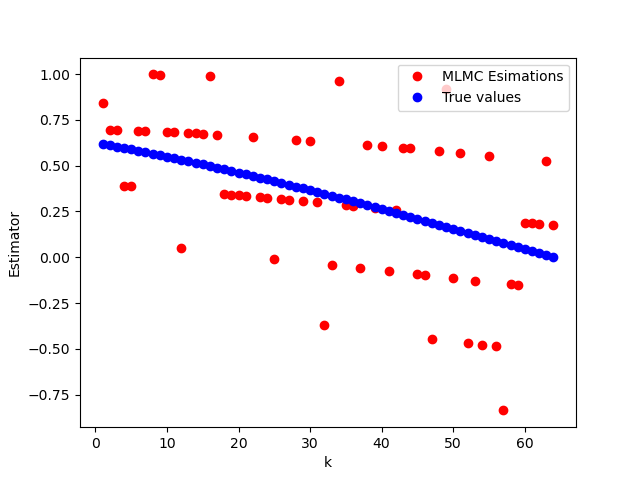
\includegraphics[width=\linewidth]{Question 8 (N=5).png}
    \caption{$N_l \equiv 5$}
  \end{subfigure}
  \begin{subfigure}[b]{0.85\linewidth}
    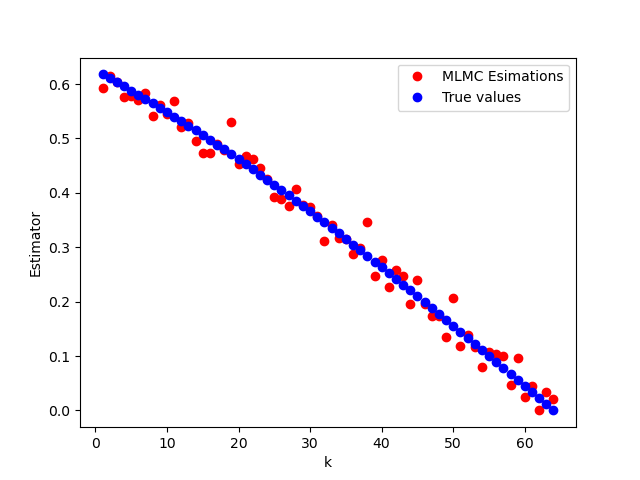
\includegraphics[width=\linewidth]{Question 8 (N=changing).png}
    \caption{$N_l=2^{L-l}$.}
  \end{subfigure}
  \caption{Estimations for $\hat\mu_{N_{1:L}}$ with $N_l = $(a) or (b) as described, for varying $k$.}
  \label{fig:Q8 Estimators}
\end{center}
\end{figure}

\begin{figure}
\begin{center}
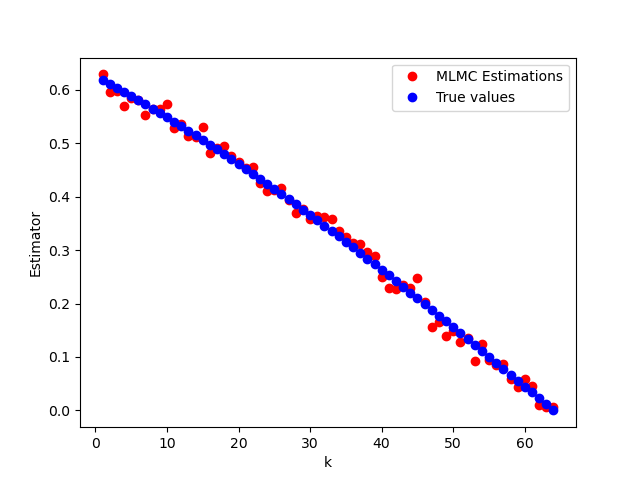
\includegraphics[width=0.85\linewidth]{Question 13 (a).png}
\caption{Estimations for $\hat\mu_{N_{1:L}}$ with $N_l $ as described in Question 13, for varying $k$.}
\label{fig:Q13 Estimators}
\end{center}
\end{figure}

\begin{figure}
\begin{center}
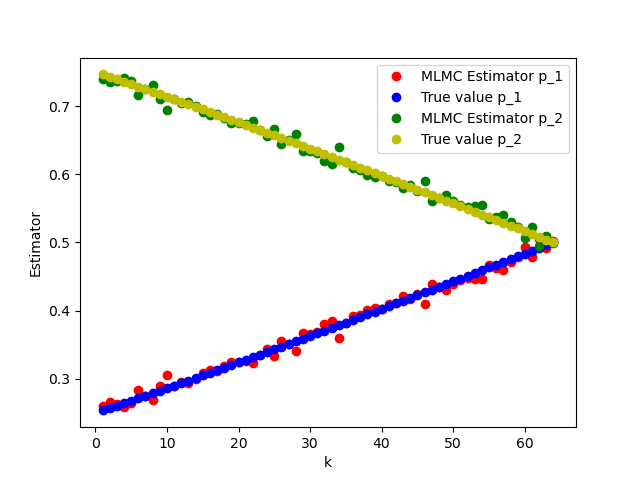
\includegraphics[width=0.85\linewidth]{Question 13 (b).png}
\caption{Estimations for $p_1(\theta)$ and $p_2(\theta)$ against the true values with $N_l $ as described in Question 13, for varying $k$.}
\label{fig:Q13 Estimators2}
\end{center}
\end{figure}














\end{document}
